% Basic LaTeX template for NE 204 lab report
%defines the type of document you will be using
%Most journals have their own style.
\documentclass[11pt]{article}

%==============================================================================
%%% Everything between the "="'s is the preamble.
%%% Define packages and meta data here

% Common packages
\usepackage{amsmath}    % Expanded math
\usepackage{amssymb}    % Expanded math symbols
\usepackage{graphicx}   % For images
%mhchem is beneficial for Nuke Eng.
%\usepackage[version=3]{mhchem} % For nuclide formatting

% All images/figures will be stored in the images folder.
% Specify that here so pdflatex knows where to look for images.
\graphicspath{{./images/}}

% Metadata
\title{Exploring with a Gaussian Distribution}
\author{Matthew Marshall}
\date{\today}
%==============================================================================

\begin{document}

% Compile metadata from preamble into a nicely-rendered title section
\maketitle

% The *'s next so section/subsection definitions suppresses numbering
% \section*{Introduction}
\section{Introduction}
\label{sec:intro}
Gaussian distribution show up all over the place in nature.
The reason for this is well known,
and often attributed to the Central Limit theorem. blah blah blah blah
\cite{clt} \cite{clt2}

We're interested in stuff. and this is a change. One more thing. Test on
branching. I am attempting something. I am here. This is new


\section{Methods}
\label{sec:meth}
Experimental procedure / set up / methods go here.


\section{Results}
\label{sec:res}
       The peak selection and fitting procedure outlined in Section~\ref{sec:meth}, resulted in a linear energy calibration of the form
\begin{equation}
E = .281*Bin + 1.81
\end{equation}
The ${133}$Ba spectrum presented in Figure~\ref{fig:BaSpec}. A comparison of the expected energy and the calibrated energies is provided in Table~\ref{tab:Comp}.


Figure \ref{fig:BaSpec} ${133}$Ba spectrum with calibration fit

\begin{figure}[!htb]
\centering
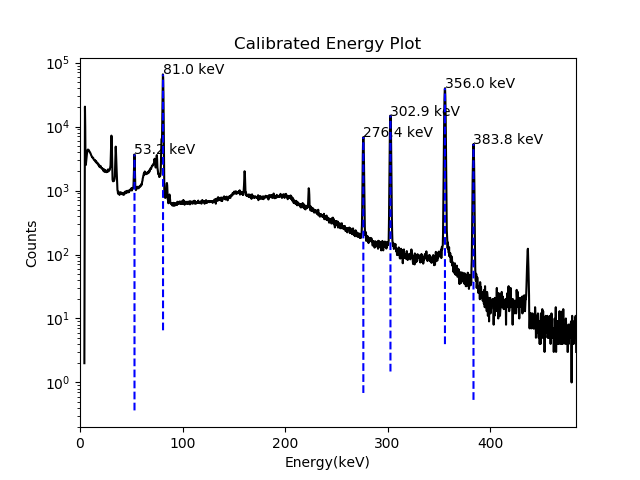
\includegraphics[width=0.5\linewidth]{images/Ba133_calibrated.png}
\caption{ ${133}$Ba spectrum with calibration fit}
\label{fig:BaSpec}
\end{figure}



\begin{table}[H]
        \begin{center}
                \begin{tabular}{ c c c c }
                        \textbf{Source} & \textbf{Energy (keV)} & \textbf{Calibration (keV)} & \textbf{abs(DeltaE) (keV)} \\
                        \hline
                        $^{133}$Ba      &      53.1622  &   53.087    & 0.074     \\5
                                                &       80.997  &       80.864  &       0.13    \\
                                                &       276.398 &       276.437 &       0.0272    \\
                                                &       302.853 &       302.805 &       0.0505   \\
                                                &       356.017 &       356.101 &       0.0968     \\
                                                &       383.851 &       383.871 &       0.0382    \\
                \end{tabular}
                \caption{Source Isotopes and Corresponding Gamma-ray energies}
                \label{tab:Comp}
        \end{center}
\end{table}


\section{Discussion}
\label{sec:disc}
	The code developed for the energy peak fitting has a number of limitations. Notabely, the code relies on finding the max point in the spectrum inorder to locate the peaks. This was only possible because of visual inspection of the spectrums confirmed that this could be done. Additionally, the width size of the peaks are predetermined meaning that if one is not careful, it is possible to combine two peaks into one or even delete a peak. The method used for fitting the peaks also requires an extra step of fitting a linear model and adding it to the gaussian fit inorder to avoid incorrect curve fitting. However, the energy calibration does fit very well. The coefficient of determination for the linear fit is .99 showing a high degree of correlation. 


% Bibliography
\bibliographystyle{plain}
% Refers to a bibtex file in the current dir named "references.bib"
\bibliography{references}

\end{document}
